\documentclass[703030]{iisreport}

% These two packages are highly recommended:
\usepackage[T1]{fontenc} % make non-ASCII characters cut&pastable in PDF
\usepackage{lmodern}     % easiest way to get outline fonts with T1 encoding
\usepackage{graphicx}
\usepackage{listings}
\usepackage{url}

\title{Documentation}
\author{Bernhard Fritz, Mike Koch, Mario Zelger}

\begin{document}
\maketitle

\begin{abstract}
  This document explains how to write IIS reports. It is written in the IIS Report style.
\end{abstract}

\section{Introduction}

Your document should begin with an introduction.

\section{Technical Content}

This is the bulk of your report, one or more sections, with nice illustrations. It is good style to cite people, not publications, as recommends \cite{Piater-2011-IISreport}. Web references should be avoided to the extent possible because they cannot usually be considered \emph{archival} \citep{Wikipedia-Archive}, and require careful assessment of reliability.

\subsection{Odometry}
For odometry we implemented a simplified approach as an alternative to the 
technique discussed in lecture. In general, robot movement can be distinguished 
between rotational and translational movement. Our idea was that if you are aware
of the robot's turn and movement speed, you have enough information to make it 
move wherever you want to. While turning/moving, the robot continuously updates its 
own estimated position and orientation. Of course due to the fixed time intervals 
there will be some small error over time but even the best odometry has troubles 
dealing with these kinds of problems.

\subsection{Generating motion commands to attain goal location}
After the first two exercises we concluded that we can no longer use the default
moving and turning robot commands ('k' and 'l') since they were very inaccurate.
So we decided to use a combination of the following commands instead:
\begin{itemize}
	\item 'w' for moving forward
	\item 's' for stopping
	\item 'i' to set a specific velocity (we used this to turn in place)
	\item 'q' for sensor measurements
\end{itemize}
These commands as well as Java's capability of letting a thread sleep for a
specific amount of time, enabled us to implement more precise motion commands.
We decided to use a design pattern called command pattern as seen in figure
\ref{img:commandpattern} to structure our code.
Following commands have been implemented:
\begin{itemize}
	\item Translation
	\item GoTo
	\item RelativeRotation
	\item AbsoluteRotation
	\item Measurement
\end{itemize}

\subsubsection{Translation}
The \emph{Translation} command can be considered as a command for relative robot
movement. As soon as the \emph{Translation} command is called we send a 'w' character
to the robot. This results in sudden forward movement of the robot. Given a
distance in cm as parameter and the robot's velocity we measured when we got the
robot, we are able to calculate the time we need to wait to send a 's' character
to the robot to make it stop. While the robot is moving we constantly keep track
of its x and y coordinates in world coordinate system.

\subsubsection{RelativeRotation}
As soon as the \emph{RelativeRotation} command is called we send an 'i' character 
with specific parameters to make the robot rotate in place counterclockwise. Given 
an angle in radiant as parameter and the robot's turn velocity we measured when we
got the robot, we are able to calculate the time we need to wait to send a 's'
character to the robot to make it stop. While the robot is turning we constantly
keep track of its angle in world coordinate system.

\subsubsection{Absolute Rotation}
\emph{AbsoluteRotation} is an extenstion of \emph{RelativeRotation} and only uses 
some math to enable us to make the robot turn to a specific angle in world 
coordinate system.

\subsubsection{GoTo}
GoTo consists of two commands: \emph{AbsoluteRotation} and \emph{Translation}. 
Given two parameters x and y (world coordinates) and the robot coordinates, we are
able to calculate the angle we need to turn the robot so that it is facing the goal
as well as the distance to the goal using trigonometry.

\subsubsection{Measurement}
The \emph{Measurement} command is used whenever we want to read sensor values. We
discovered that only three of five sensors are actually working:
\begin{itemize}
	\item front left sensor
	\item front middle sensor
	\item front right sensor
\end{itemize}
The \emph{Measurement} command is exclusively invoked by the \emph{SensorManager}
which is responsible for parsing received sensor data, calculating an average estimate
of sensor values as well as notifying observers about imminent obstacles.

\begin{figure}
	\centering
	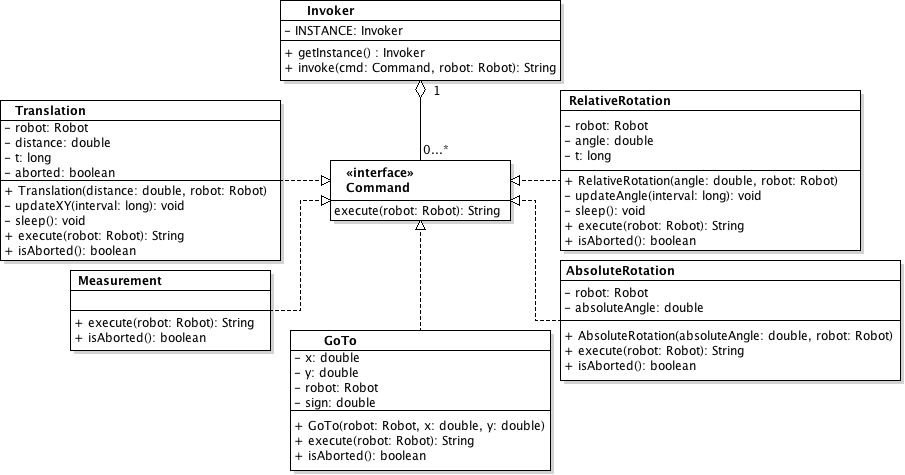
\includegraphics[width=\textwidth,height=\textheight,keepaspectratio]{commandpattern.png}
	\caption{Command pattern}
	\label{img:commandpattern}
\end{figure}

\subsection{Obstacle avoidance} \label{obstacle_avoidance}
To avoid obstacles we needed a way to keep track of sensors while moving. At
first we used a Java thread to move and poll the sensors at the same time. This
didn't work too well since there should always be some delay between two robot
commands. That is why we decided to try a different approach. Since it is not
necessary to poll the sensors all the time (e.g. turning in place), we only
focused on polling the sensors while moving. We used a design pattern called
observer pattern as seen in figure \ref{img:observerpattern} to conveniently let
all observers know if an obstacle was detected or not.

\begin{figure}
	\centering
	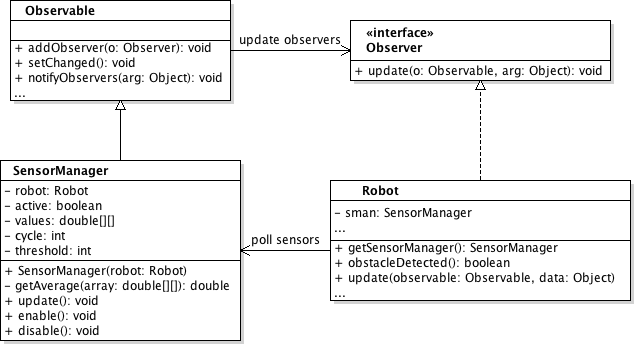
\includegraphics[width=\textwidth,height=\textheight,keepaspectratio]{observerpattern.png}
	\caption{Observer pattern}
	\label{img:observerpattern}
\end{figure}

\noindent If an obstacle was detected the current \emph{Translation} command 
will be aborted and our obstacle avoidance algorithm will be started:

\begin{lstlisting}[mathescape]
sign = 1;
while(Goal is not reached) {
  Turn towards goal;
  Move towards goal;
  if(Moving is aborted) {
    Turn sign*90$^{\circ}$;
    Move 30 cm;
    if(Movement is aborted) {
      sign *= -1;
    }
  }
}
\end{lstlisting}

\noindent Essentially this algorithm is also known as "Bug 0" algorithm as seen in \citep[7]{bug-algorithms}

\subsection{Color correction and beacon detection}
For the color correction and in addition the beacon detection we used the 
\textit{Color Blob Detection} example included in the OpenCV library \\(\url{http://opencv.org/downloads.html}).
In the example code there is a class \textit{ColorBlobDetector} which includes
the contour calculation for a specifig HSV color. We used that class for finding
the contours of our coloured balls and beacons. \\
The beacon contours we defined as two rectangles, one above the other, having
a greater height than width. \\
After we filtered that contours out of our image the remaining contours must be
the balls the robot can see from it's position. \\
The beacon detection had cost us a lot of time because we had many problems
with the different colours in different lighting positions. This was our main problem
implementing a correctly working beacon detection.

\subsection{Self-localization}
The self-localization is done like we heard in the lecture. We calculate a homography
matrix from a given chessboard picture. With that matrix and the respective OpenCV
functions we can easily calculate the distance from the robot to a beacon for example. \\
The self-localisation (only position without the angle) is done with the following algorithm:

\begin{lstlisting}[mathescape]
r1 = distance to beacon1;
r2 = distance to beacon2:
c1 = circle with radiance r1;
c2 = circle with radience r2;
p[2] = intersection points of c1 and c2;
pos = point out of p[2] which is inside the workspace;
\end{lstlisting}

\noindent This algorithm works since we know the boundaries of the robots workspace. \\
The robots angle calculation was quite more difficult. In the end we did it similar
to the algorithm we have learned in the lecture. We calculated the linear equation
for the line between the two beacons. With that equation we get the intersection point
of that line with the robots line of sight. Including one of the two beacons and the distance
between the beacon and the robot we have a triangle. From that triangle we know
all three sides so we can calculate the wanted angle with the law of cosine. \\
This calculation in combination with mostly inaccurate beacon detection caused also
a lot of problems. In the end we fixed that problems and most of the time the
self-localization worked quite fine.

\subsection{Algorithm for caging a ball with and without obstacles}
Our algorithm for caging a ball without obstacles looked like the following:

\begin{lstlisting}[mathescape]
while (no more balls at the workspace) {
  Search for 2 or more beacons;
  while (not 2 or more beacons found)  {
    Explore the workspace;
    Search for 2 or more beacons;
  }
  Do self localization;
  Search for a ball;
  while (no ball found) {
    Explore the workspace;
    Search for a ball;
  }
  Drive to the ball with distance - 5cm;
  Catch the ball;
  Go to the pre-defined target position.
  Release the ball;
}
\end{lstlisting}

\noindent For the algorithm with obstacles we simply added the obstacle avoidance described
in section~\ref{obstacle_avoidance}.

\subsection{Strategy for the tournament}
Out strategy for the tournament was to catch all the balls in a short time without
hitting the other robot. Since the different lighting conditions we had problems with
the beacon detection and the self-localization. We did some nice tries with our robot but
in the end it mostly detected the wall as an obstacle and did erratic movements. \\
The tournament still made a lot of fun and the big challenge with all robots driving
at the same time in that small workspace was the highlight.

\subsection{Miscellaneous}
  \subsubsection{User interface}
  \subsubsection{Work contribution breakdown}


\section{Conclusions}

Your document should conclude with a summary of the highlights, and any conclusions to be drawn.

\bibliography{refs}

\end{document}
